\section{Results}

Using the benchmarked ice flow model of Greenland, in this section, the impact of varying climate scenarios on the GrIS as well as realistic projections over the next millennium are discussed. 

\subsection{Sensitivity to synthetic climate change}

% How does the volume of the Greenland ice sheet depend on changes in climate? (5 points)
% How are differences in temperature different from changes in precipitation? (5 points)
% How do different regions respond to climate change? (5 points)
% How fast does ice grow or retreat? (5 points)
% Does a doubling in the temperature anomaly cause a doubling in ice loss (linearity of response)? (5 points)
% How linear is the response to precipitation changes? (5 points)

Two diverging climate scenarios are applied to the ice flow model, i.e., the climate fields used to compute the SMB are altered by varying scaling factors.

\begin{itemize}
	\item \textbf{glacial-climate}: A glacial climate is marked by cold temperatures and low precipitation. Accordingly, the mean temperature is decreased by \(\Delta\mean{T} = \SI{-13}{\celsius}\) and mean precipitation is adjusted\footnote{The scaling of the precipitation's latitudinal gradient is updated to be consistent with the new mean precipitation.} by \(\Delta\mean{P} = \SI{-4}{\mm\per\day}\) compared to the climate fields calculated from the parametrizations in \cref{tab:smb}.
	\item \textbf{warm-climate}: To include a contrary scenario, this warm, moisture-rich climate is defined by \(\Delta\mean{T} = \SI{+12}{\celsius}\) and \(\Delta\mean{P} = \SI{+4}{\mm\per\day}\).
\end{itemize}

Temperature influences the atmosphere's capacity to hold water vapour, changes evaporation rates and circulation patterns, hence, in this climate scenarios, both fields are altered simultaneously. The GrIS model runs for \SI{25000}{\year}, however, only the first \SI{20000}{\year} are considered in the following as this time interval is sufficient for the ice sheet to reach an equilibrium state. The simulations are initialized with present-day ice topography, and the model results based on the SMB characterized in \cref{sec:smb} act as \textbf{reference}.

\begin{figure}
	\centering
	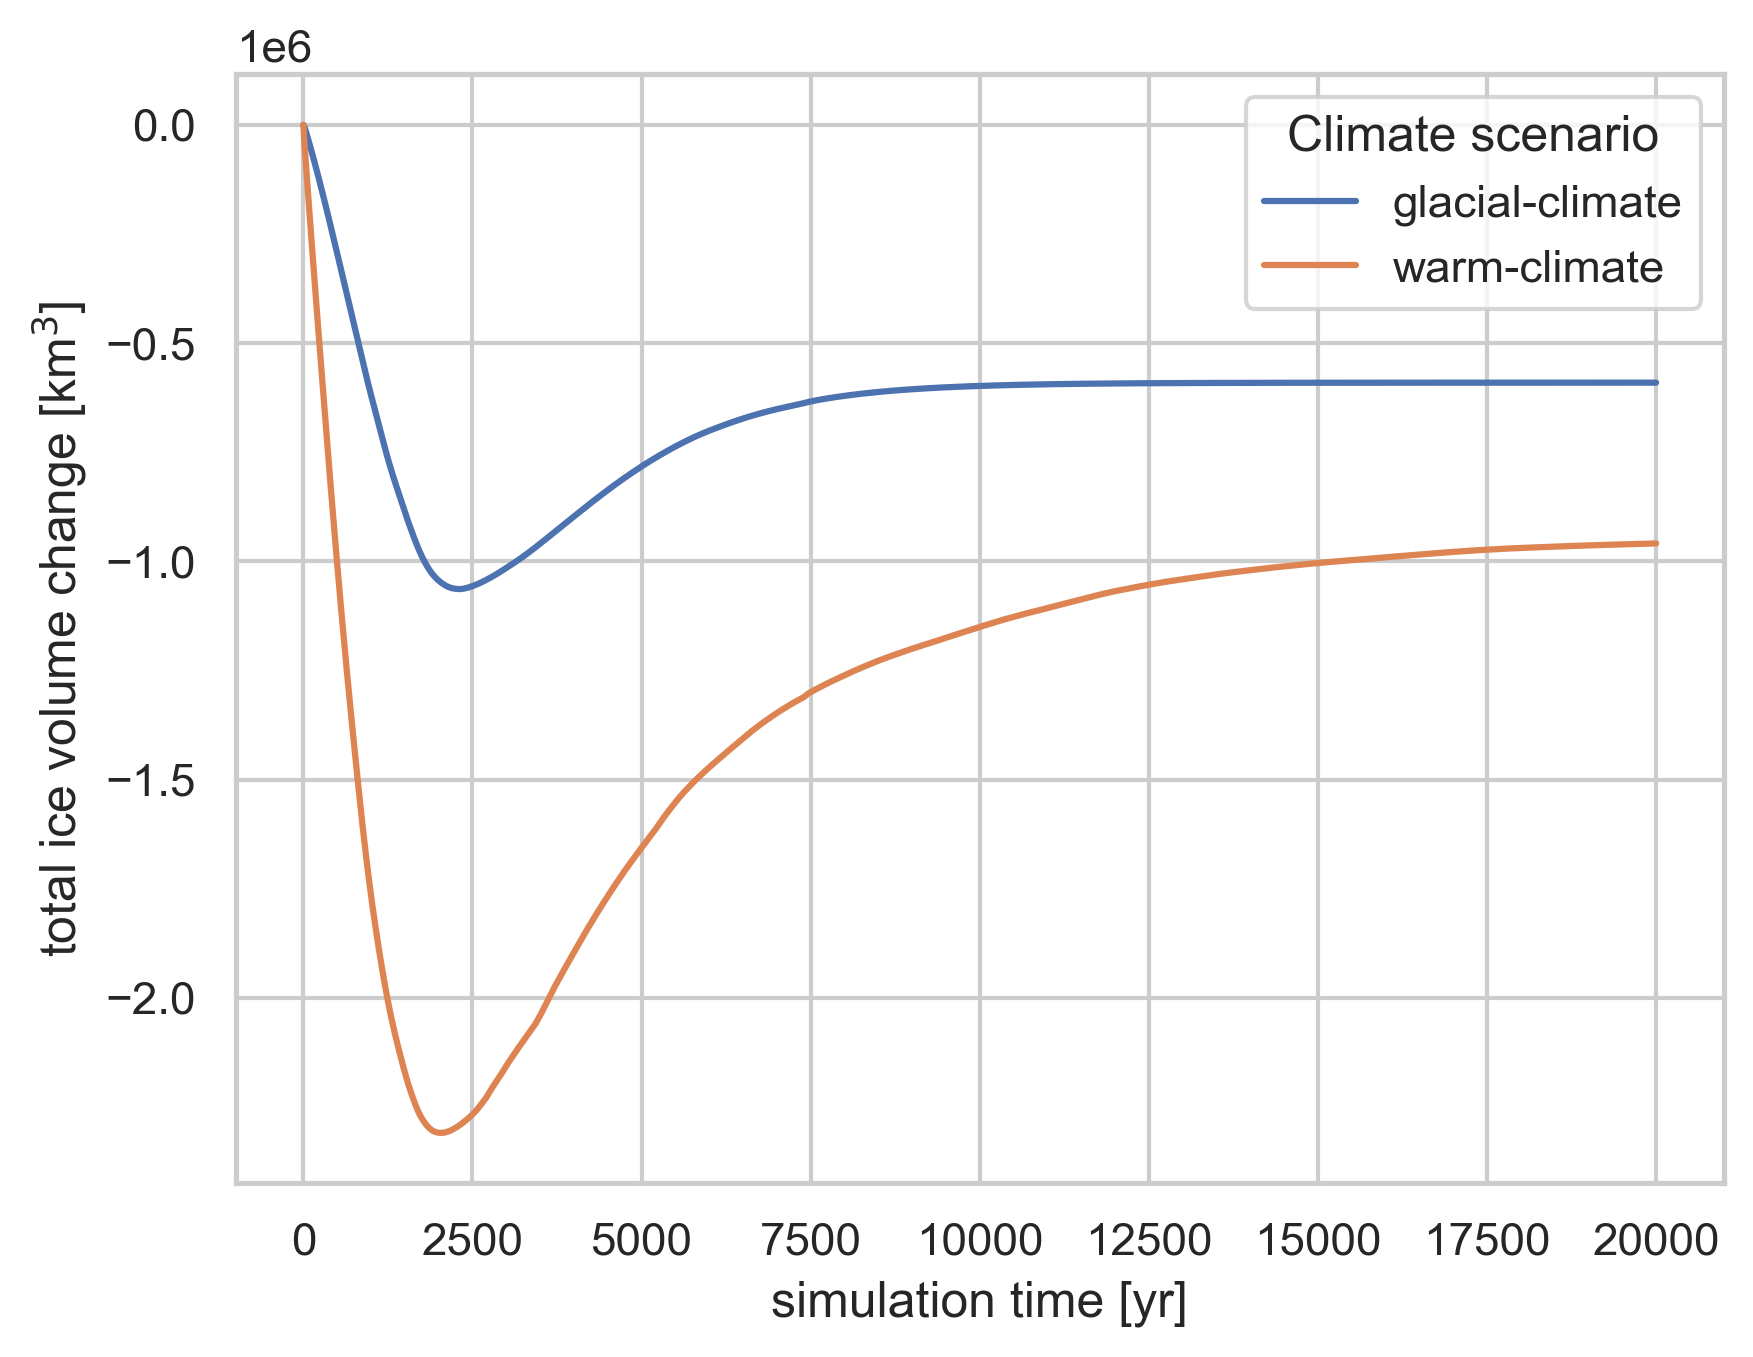
\includegraphics[width=0.7\textwidth]{../climate-anomalies/figs/ice-volume-change.png}
	\caption{Change of the total GrIS ice volume in respect to the reference simulation for both climate scenarios}
	\label{fig:scenarios-icevol-change}
\end{figure}

Both climate scenarios ultimately reach equilibrium states of reduced GrIS volume compared to the reference model run, however, as expected, of the two scenarios, the glacial climate succeeds in maintaining the larger ice volume as shown in \cref{fig:scenarios-icevol-change}. Here, the \textit{continuous} difference in ice volume with respect to the reference simulation is plotted, thus, it is important to note that the reference shows a total ice volume gain of \SI{3.32e6}{\km^3} after \SI{5000}{\year} (reaching an equilibrium), which is roughly a doubling of the initial ice volume.
Although one could argue that a reference should not display such an increase in ice volume, the reference's parametrization is based on published values as well as reanalysis data, thereby pointing towards limitations in trusting absolute values derived from this (rather simple) GrIS model. Interestingly, the ice volume change is characterized by a minimum in the early stage of the simulation of both climate scenarios. The glacial climate is slower in reaching an equilibrium state, hence, initially the difference in ice volume between the glacial scenario and the reference is larger. The same holds true for the warm climate, however, here melting dominates the ice volume change at first until the flow of ice compensates, and thus it takes even longer to establish an equilibrium.

\begin{figure}
	\centering
	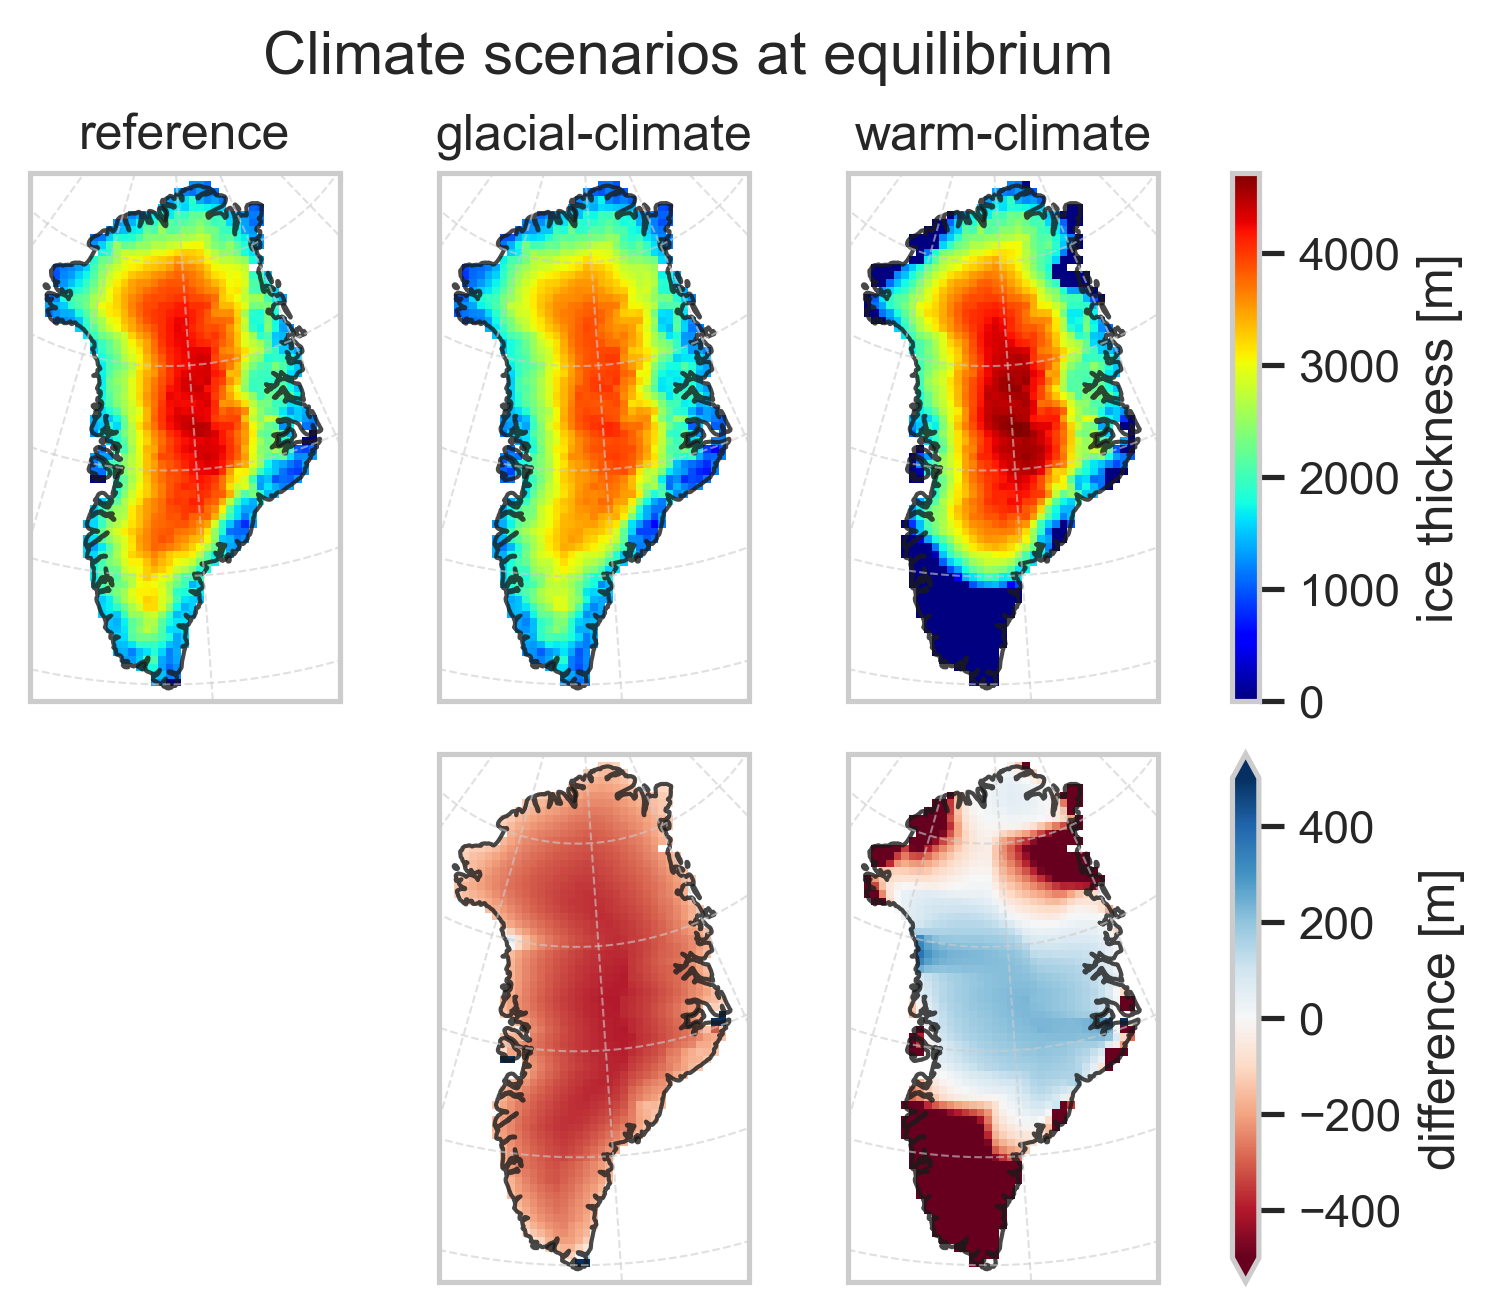
\includegraphics[width=0.7\textwidth]{../climate-anomalies/figs/ice-thickness-maps.png}
	\caption{Ice thickness of final simulated time step; difference between climate scenario and reference below the respective scenario}
	\label{fig:scenarios-thick-maps}
\end{figure}

To further investigate this state, \cref{fig:scenarios-thick-maps} reveals the difference in spatial distribution of ice thickness among the climate scenarios. The glacial conditions yield an ice sheet with reduced elevation, yet consistent structure, when compared to the reference, indicating that the glacial climate simply cannot sustain such an elevated ice sheet due to low accumulation rates and loss of ice through transport towards the coastline (where the implemented \enquote{calving} makes the ice disappear). The warm climate conditions show a pronounced region in the south-west where the ice sheet completely melts, on top, two areas in the north experience noticeable ice loss with respect to the reference state---on the contrary, central Greenland is characterized by an increase in ice elevation. Here, temperatures are still below freezing and thus enable accumulation, which is enhanced due to raised mean precipitation. Put together, the warm climate manages to aggregate the highest ice sheet although regions closer to the coastline experience strong ablation.

To untangle the combined effects of temperature and precipitation changes, the low numerical complexity of the GrIS allows running multiple perturbed simulations in an acceptable amount of lifetime. Following an approach by \textcite{born2019}, the ice flow model is either initialized with anomalous temperature fields only (\(\Delta\text{T}\)) or with both anomalous temperature and precipitation fields (\(\Delta\)T\&\(\Delta\)P). The temperature anomalies are uniformly spaced from \SIrange{0}{12}{\celsius} and the precipitation anomalies from \SIrange{0}{1}{\mm\per\day}, resulting in a total of eight perturbed simulations, which run until an equilibrium state is reached. The anomaly ranges are roughly extrapolated from a projection of the Norwegian Earth System Model (NorESM) for 2100 CE provided in the course. Here, an increase in mean annual temperature of \(\Delta\mean{T} = \SI{3.8}{\celsius}\) corresponds to a positive precipitation anomaly of \(\Delta\mean{P} = \SI{0.2}{\mm\per\day}\). 

As expected, \cref{fig:anom-scatter} shows that the total ice volume generally decreases with larger temperature anomalies, regardless of whether precipitation perturbations are applied or not. Accordingly, \(\Delta\)T and \(\Delta\)T\&\(\Delta\)P show a negative curvature, and in both cases no linear relation between temperature anomaly and ice volume change is identifiable. This non-linearity is most-likely caused by positive feedback mechanisms, such as the SMB–elevation interaction introduced in \cref{sec:intro}.

\begin{figure}
	\centering
	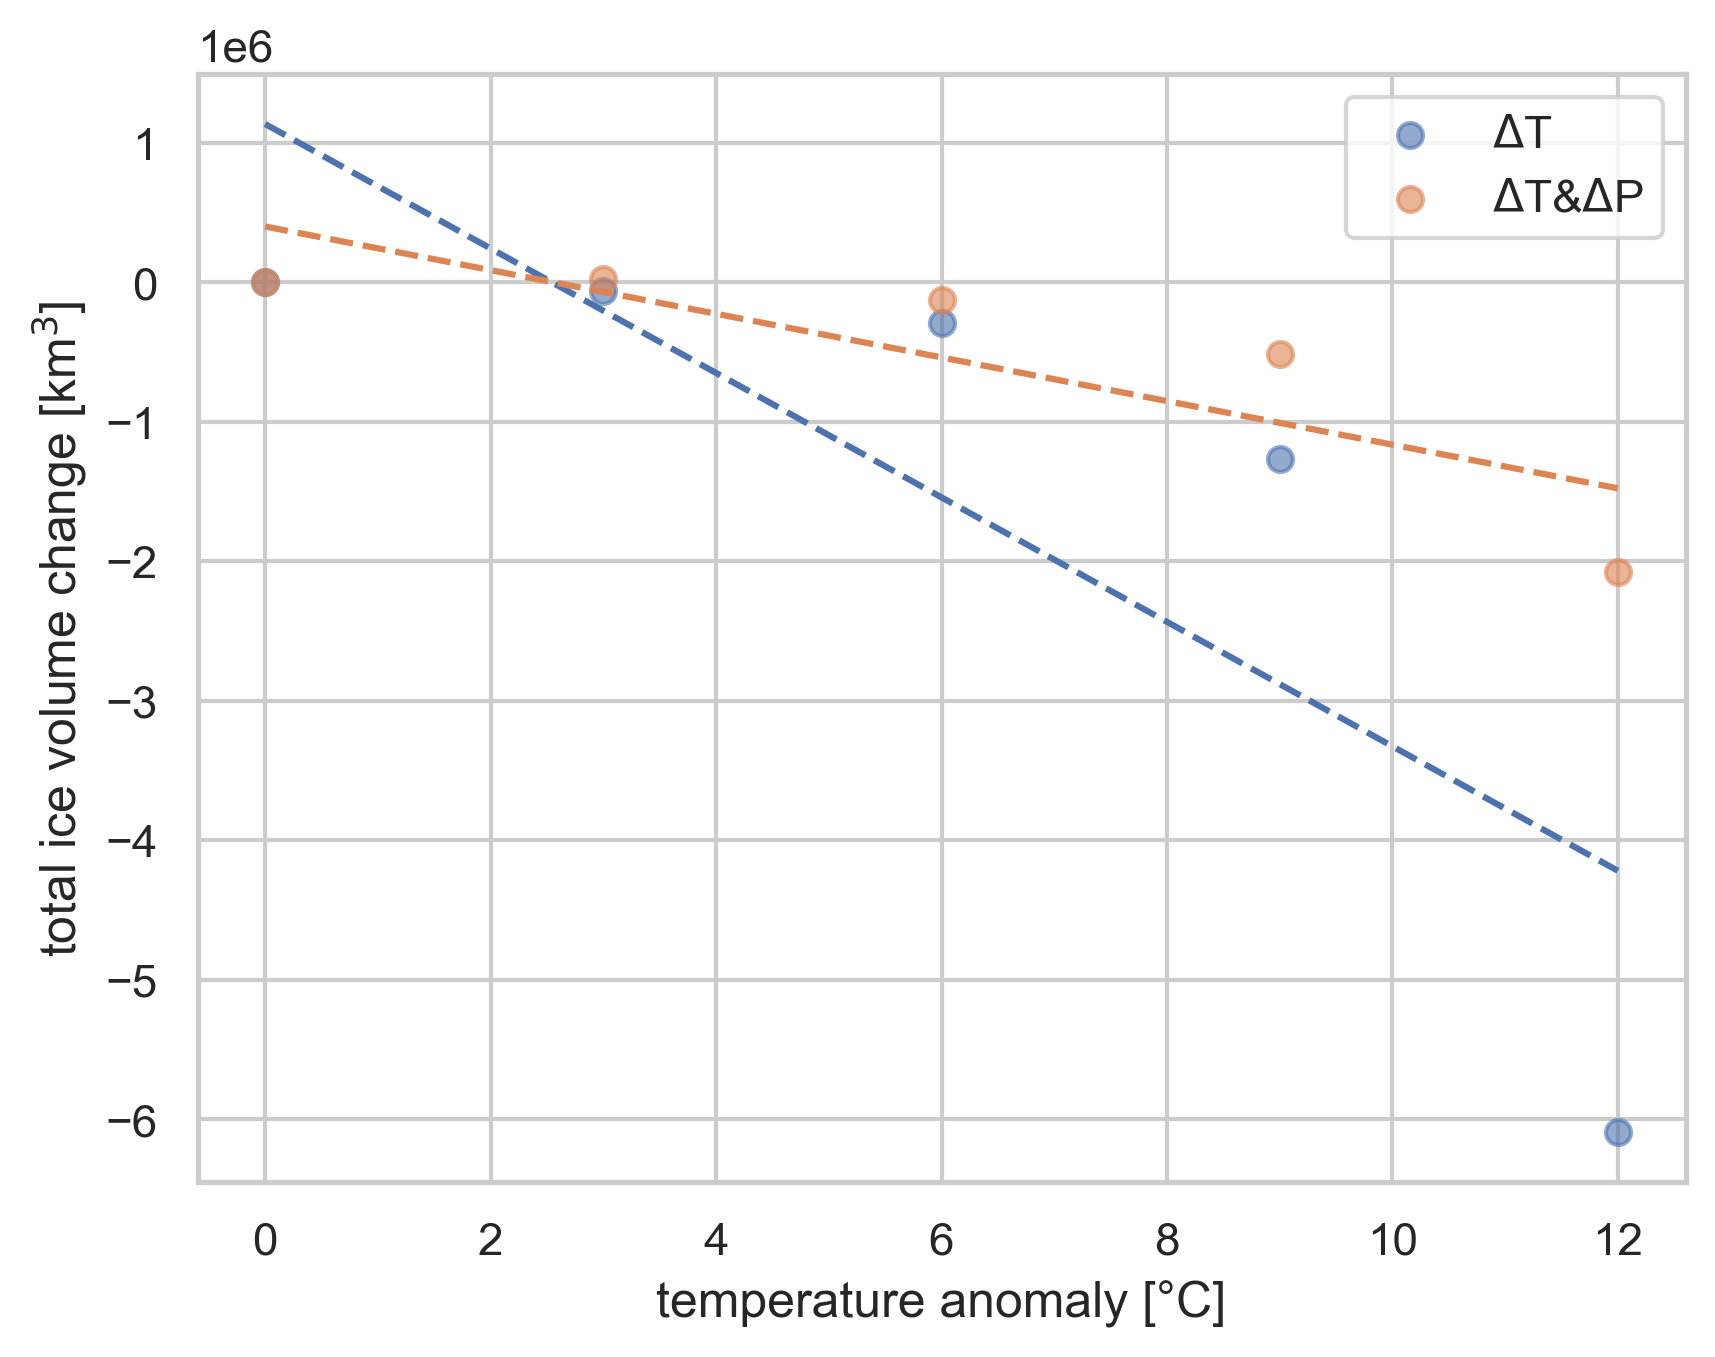
\includegraphics[width=0.7\textwidth]{../climate-anomalies/figs/icevol-deltat.png}
	\caption{Change in total ice volume as a function of temperature anomaly. Either perturbation of temperature field only (blue) or perturbation of both temperature and precipitation field (orange) is applied to initialize GrIS model; dashed lines represent linear fits.}
	\label{fig:anom-scatter}
\end{figure}

\begin{figure}
	\centering
	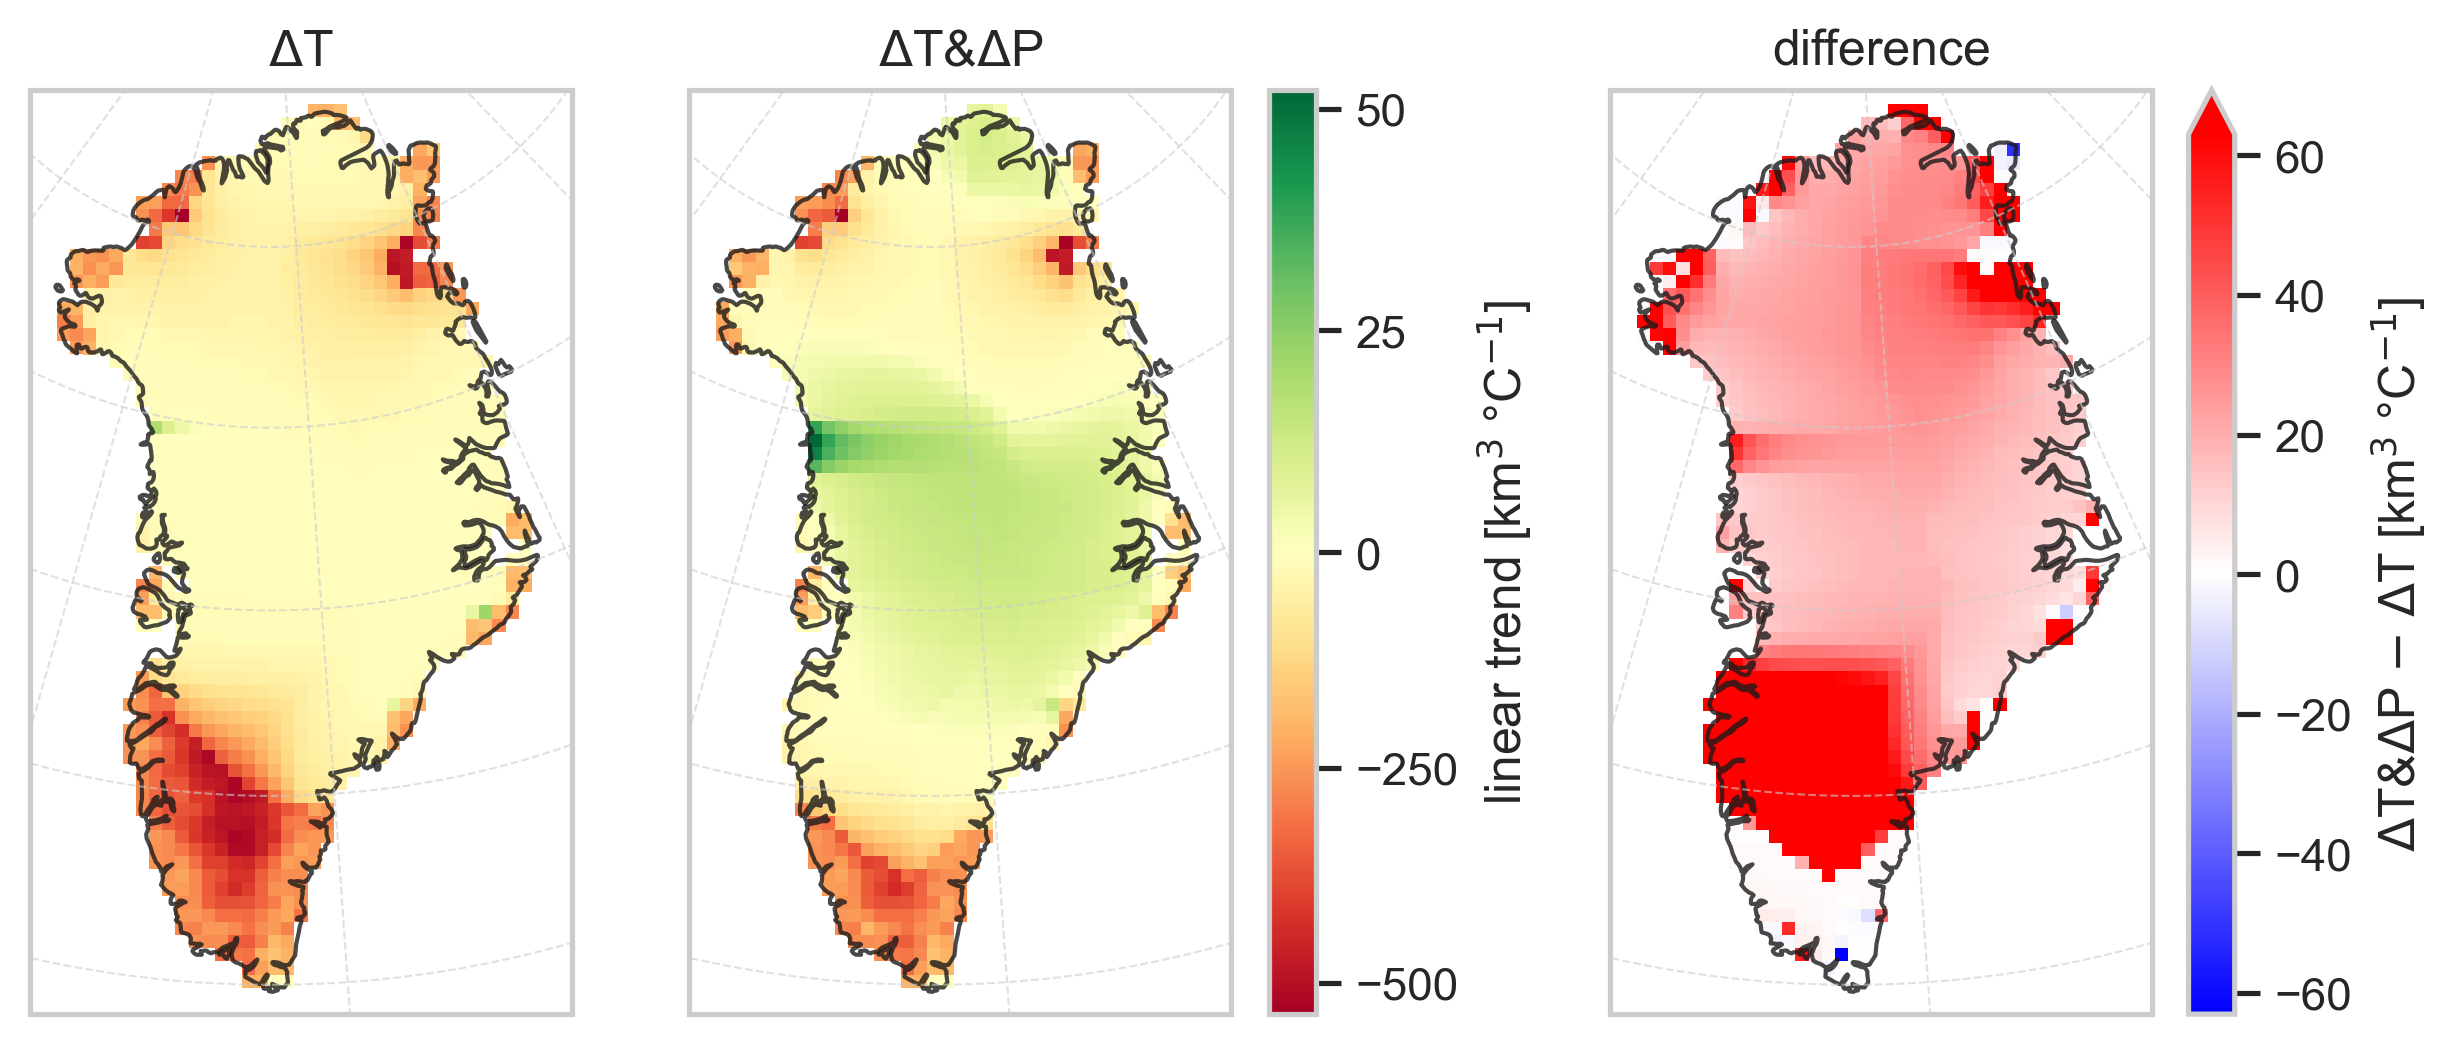
\includegraphics[width=0.85\textwidth]{../climate-anomalies/figs/linear-trend.png}
	\caption{\textit{Left:} Spatial distribution of the linear trend in total ice volume change as a function of temperature anomaly. Note the non-linear colour scale. \textit{Right:} Difference of initializing simulations with anomalous temperature alone (\(\Delta\)T) and with both temperature and precipitation anomalies (\(\Delta\)T\&\(\Delta\)P).}
	\label{fig:anom-maps}
\end{figure}

Although the change in total ice volume does not follow a linear trend, generally speaking, the sign of the slope reveals whether the ice volume in- or decreases with respect to the magnitude of perturbations. Repeating the regression for each grid point of the model's spatial domain yields maps of the linear trend for \(\Delta\)T and \(\Delta\)T\&\(\Delta\)P, presented in \cref{fig:anom-maps}. If the GrIS model is perturbed with temperature anomalies only, the linear trend is predominantly negative, in particular, large negative slopes are observed in the south-west area. Including precipitation anomalies results in an increase of ice volume with higher temperatures in central Greenland. The difference of \(\Delta\)T and \(\Delta\)T\&\(\Delta\)P is overall positive, implying that more precipitation (and higher accumulation rates) can counteract increased melting in some areas. Interestingly, the pronounced difference in the south is caused by transport of ice from the elevated (growing) ice sheet in central Greenland towards the southern ablation zone, only possible in the case of \(\Delta\)T\&\(\Delta\)P. These results also align with the previous analysis of the climate scenarios and further explain how the warm climate is able to sustain a large ice sheet in the central region.

\subsection{Future of the Greenland ice sheet}

% Simulation and documentation (with figures) of the GrIS response to climate change until the year 3000 with an idealized climate forcing. (10 points)
% Simulation and documentation of the GrIS response to climate change until the year 3000 with the provided climate fording. (10 points)
% How can the findings from the idealized simulations of exercise 2 help to interpret the new results? (10 points)
% How does the rate of ice loss compare to published estimates? (5 points)
% Is (the rate of) ice loss similar in different regions? (5 points)

The entire GrIS holds \SI{7.4}{\m} of sea level equivalent \parencite{morlighem2017} and is sensitive to changing climate conditions. In this section, the response of the GrIS to varying climate forcings in this millennium is simulated. Two different approaches of acquiring the temperature and precipitation fields, that in turn are used to calculate the annual SMB, are applied.
\begin{itemize}
	\item The NorESM can be used to derive daily temperature and precipitation anomalies for 2100 CE, which, combined with the present-day climatology, yield climate fields for that particular year. To obtain a continuous forcing, the anomalies are scaled by a climate index, which is presented in \cref{app:forcing-noresm}. The scaling processes to calculate the climate fields are omitted, rather, the climate forcing is determined directly from results of complex climate models. Their output is provided as part of the course, and the corresponding climate forcing is labelled as \textbf{NorESM} in the following.
	\item Secondly, a rather idealized warming scenario is achieved by maintaining the SMB scalings (\cref{tab:smb}), and adjusting the respective parameters to obtain the desired climate forcing. To establish a warming scenario analogous to the NorESM forcing, the temperature is increased by \(\Delta\mean{T}=\SI{12}{\celsius}\) (refer to \cref{app:forcing-idealized} for further details). In an alternative warming scenario, the temperature is raised by \(\Delta\mean{T}=\SI{4}{\celsius}\) to receive a climate forcing that corresponds to late-21\textsuperscript{st}-century conditions, following an approach by \textcite{greve2022}. The temperature field scaling is kept constant throughout the simulation, and the respective warming scenarios are labelled as \textbf{idealized\_<\(\Delta\mean{T}\)>}.
\end{itemize}

\begin{figure}
	\centering
	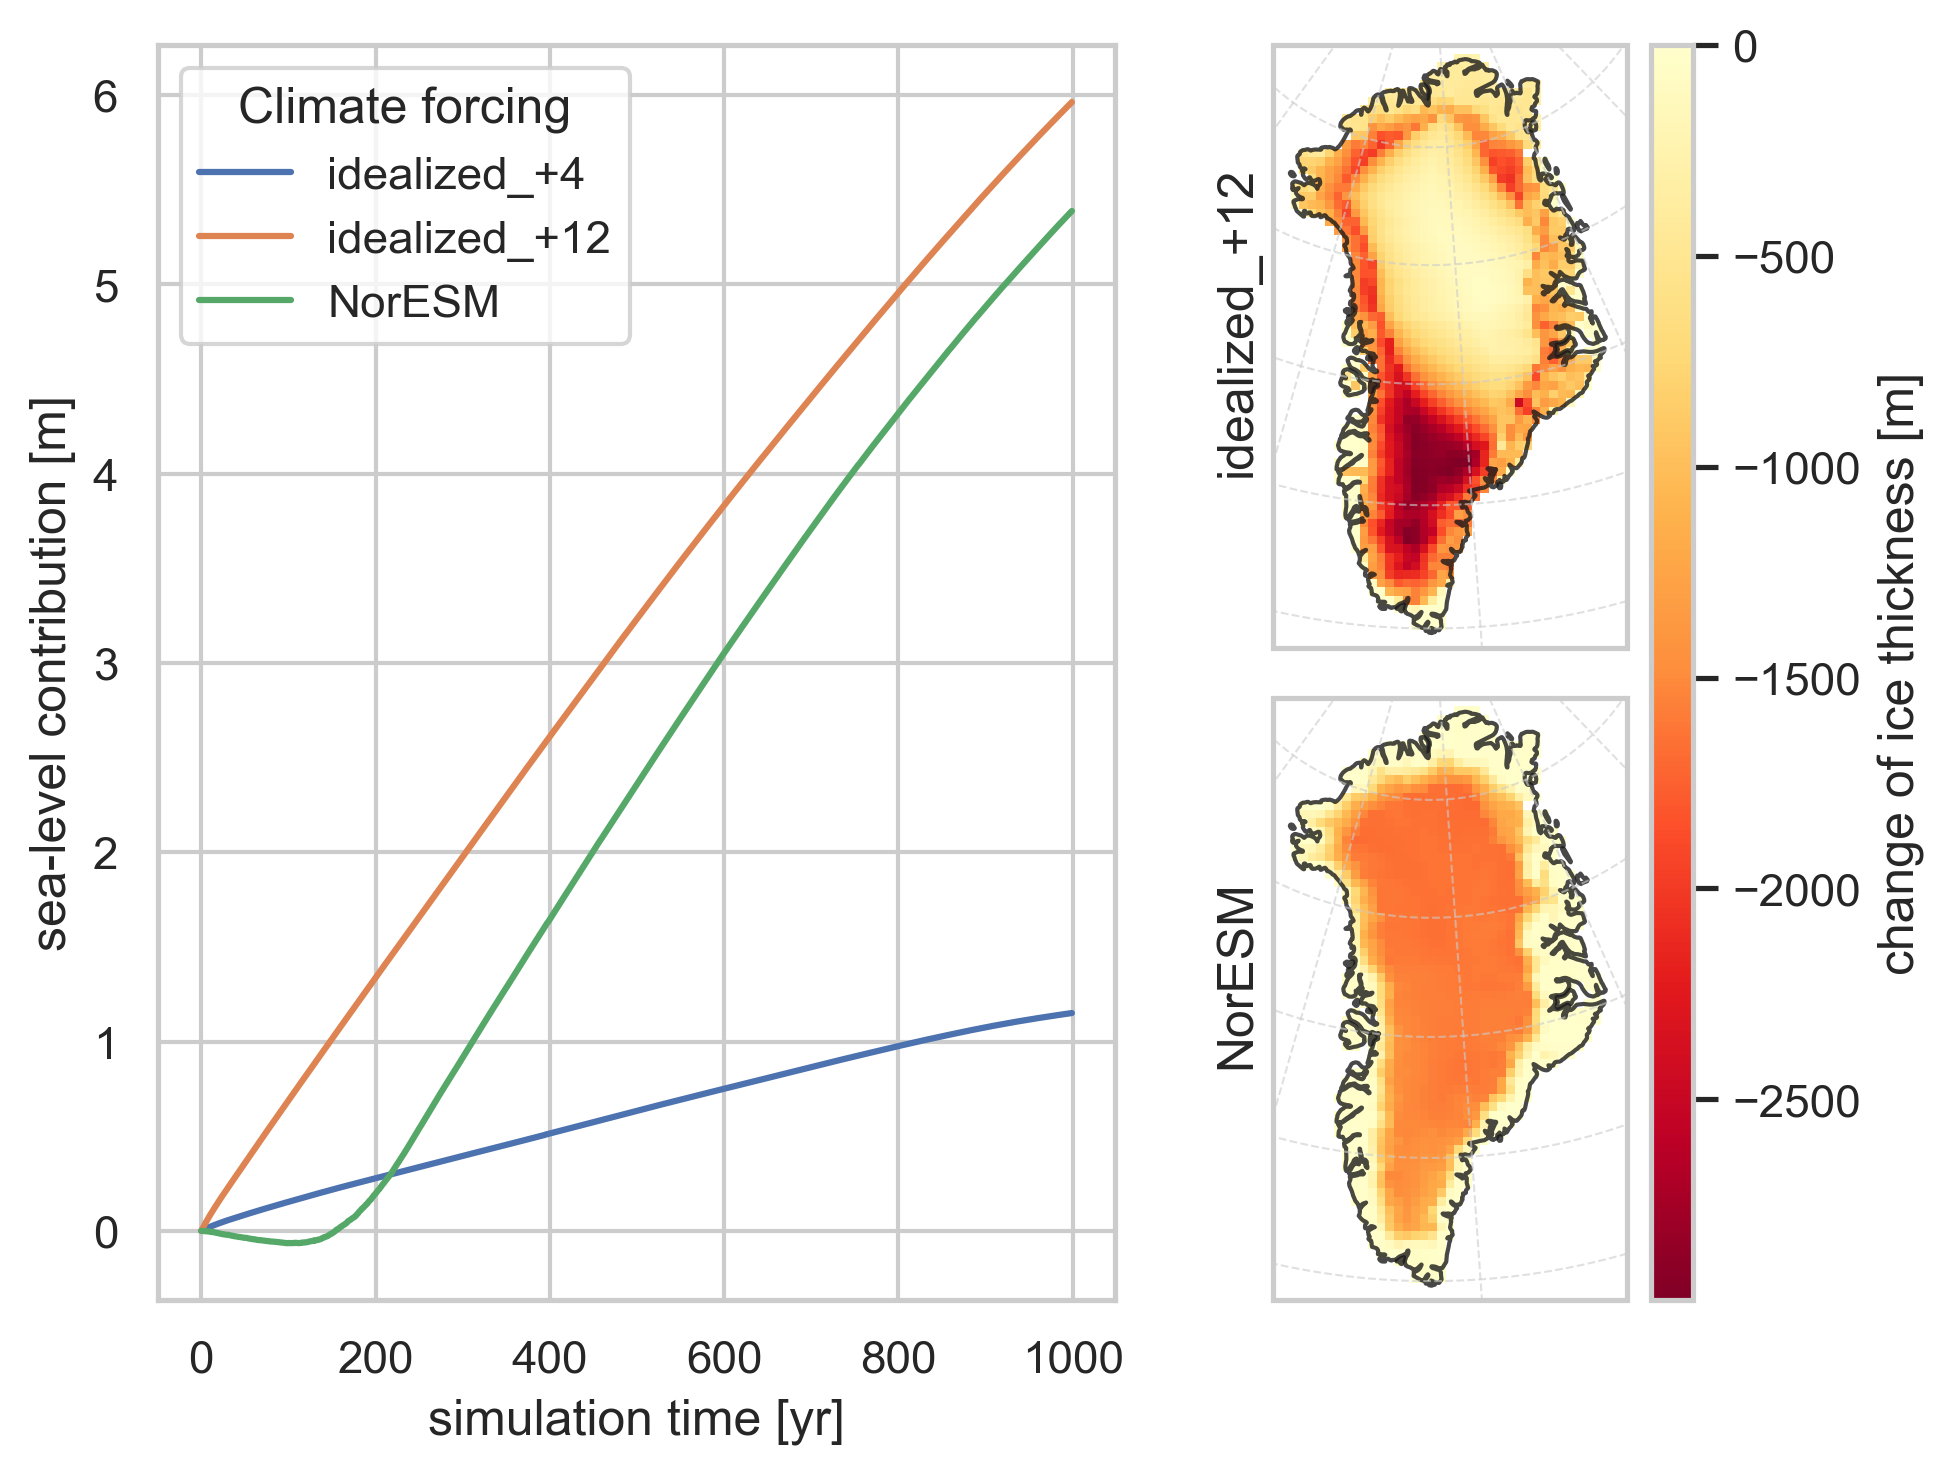
\includegraphics[width=0.8\textwidth]{../global-warming/figs/sea-level-contribution.png}
	\caption{\textit{Left:} Accumulated sea-level contribution until 3000 CE depending on climate forcing scenario with respect to the reference simulation (idealized\_*) or the initial GrIS state (NorESM). \textit{Right:} Difference in ice thickness at final time step of (\textit{top}) strong idealized warming and reference, and (\textit{bottom}) NorESM forcing scenario and present-day ice thickness.}
	\label{fig:warming-sea-level}
\end{figure}

The resulting effects of the climate forcings on the GrIS during this millennium are presented in \cref{fig:warming-sea-level}. The simulated ice volume changes are counted positively for loss and expressed as sea-level contribution. By 3000 CE, the GrIS contributed \SI{1.15}{\m} (idealized\_+4), \SI{5.39}{\m} (NorESM) or \SI{5.96}{\m} (idealized\_+12) to global sea-level rise, depending on the warming scenario. For the more pronounced warming scenarios (NorESM and idealized\_+12), this is almost equivalent to a complete ablation of the GrIS, a result confirmed by \textcite{aschwanden2019}. The authors applied also an extreme warming scenario, namely, extrapolating the increasing temperature trend up until 2500 CE, after which they kept the temperature constant, and observed complete melting of the GrIS following the RCP8.5 scenario. The mass loss of the moderate climate forcing (idealized\_+4) is consistent with the results of \textcite{greve2022}, who found the GrIS's sea-level contribution to amount to \SI{1.79 +- 0.8}{\m\ SLE} for RCP8.5 by 3000 CE.

\begin{figure}
	\centering
	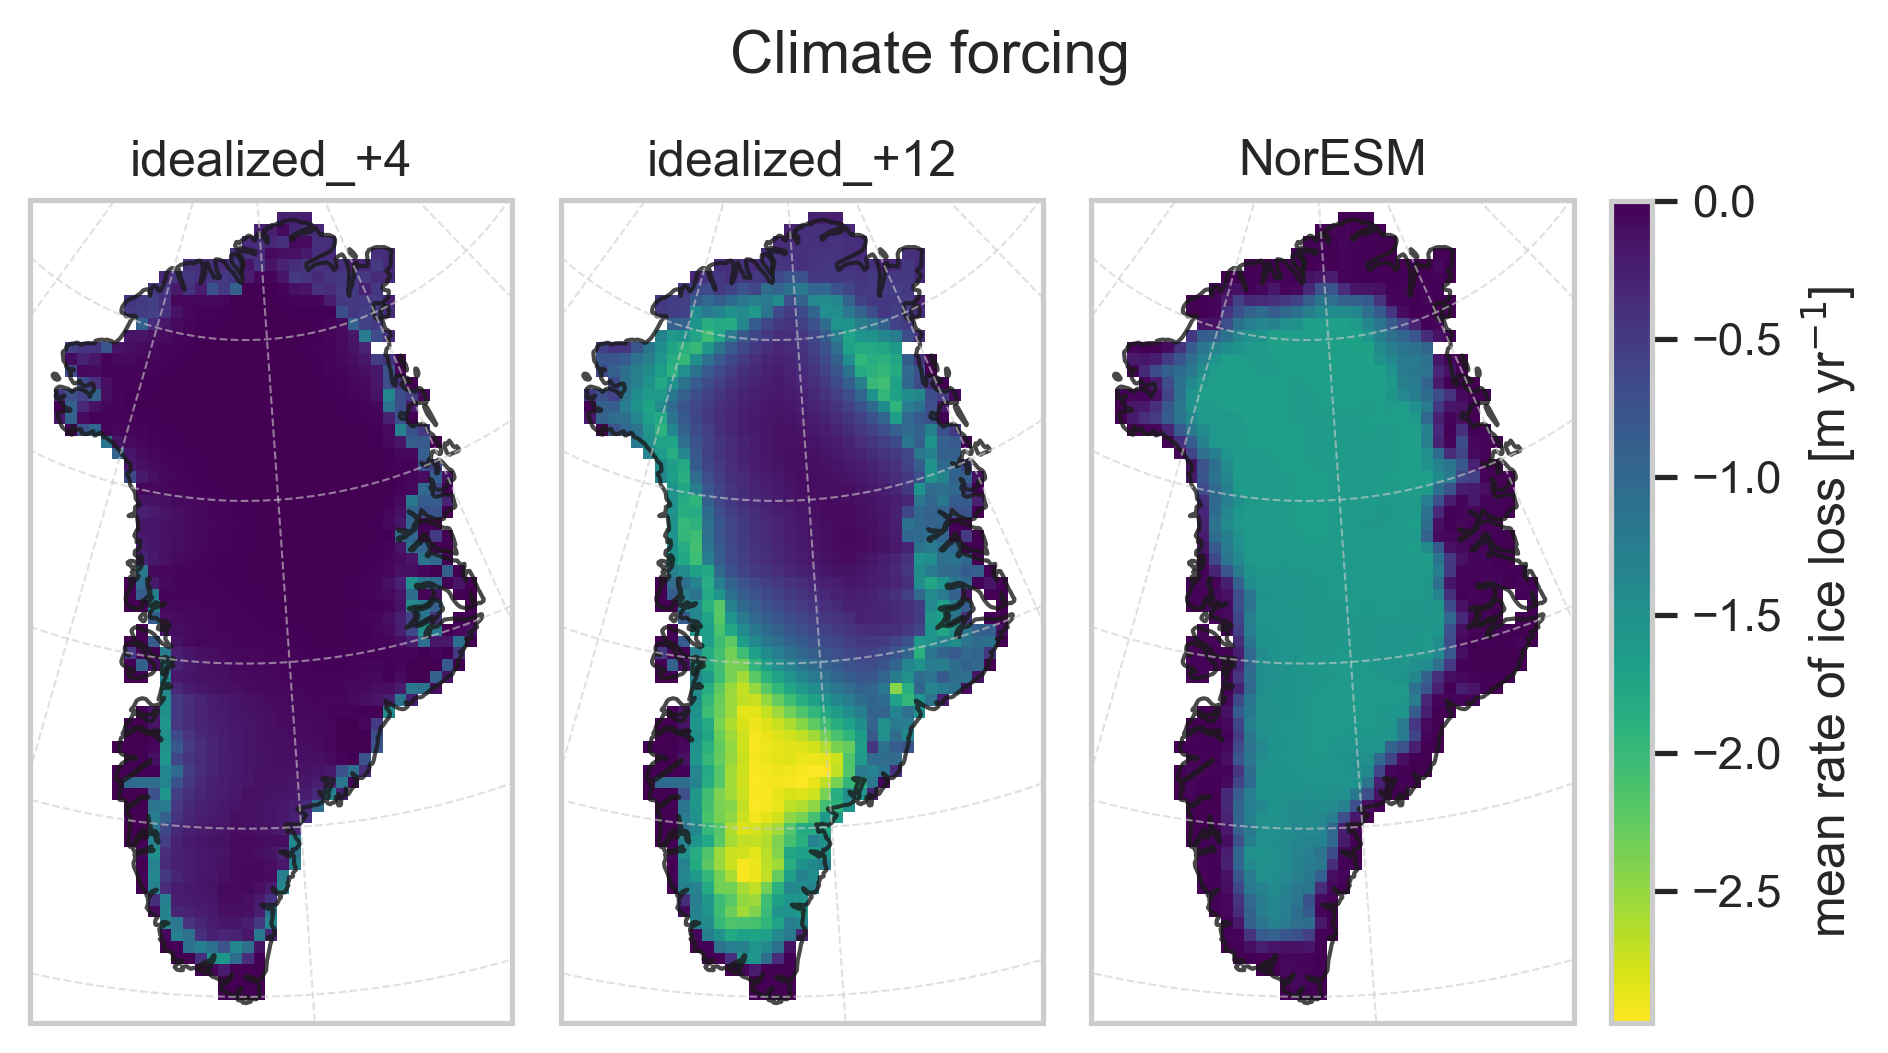
\includegraphics[width=0.85\textwidth]{../global-warming/figs/ice-loss-rate.png}
	\caption{Spatial distribution of time-averaged gradient of ice thickness change for different climate forcing scenarios}
	\label{fig:rate-ice-loss}
\end{figure}

Although the total ice loss of idealized\_+12 and NorESM turns out to be roughly the same, spatially resolving the change in ice thickness (\cref{fig:warming-sea-level}) reveals a differing situation: While the NorESM forcing scenario leads to relatively uniformly-distributed ice loss, the idealized warming shows an area of pronounced melting in the southern part of Greenland, yet leaving the central ice sheet more or less untouched. Furthermore, if focussing on the mean rate of ice loss in \cref{fig:rate-ice-loss}, an analogous structure is observed for the strong warming scenarios: Again, the idealized\_+12 forcing displays the largest (mean) rates of ice loss in the southern region with more than \SI{-2.5}{\m\per\year}, while the NorESM forcing leads to consistent ice loss rates of around \SI{-1.5}{\m\per\year} for most of the GrIS. Finding such similarities in the spatial distribution between the ice loss rate averaged over the entire duration of the simulation and the ice thickness change at the end of the simulation is also linked to the fact that the accumulated sea-level contribution is approximately linear in time (except for the NorESM forcing in the beginning of the simulation). The strong melting in southern Greenland might not be present in the NorESM forcing scenario as it is counteracted by high precipitation rates found in that region (see \cref{fig:21c-warming}), while the climate field scaling processes used in the idealized warming scenarios fail to reproduce such strong, localized precipitation signals. The idealized\_+4 warming scenario shows moderate ice loss at the edges of the GrIS, while the centre is mainly unaffected, which matches the simulated ice thickness maps found in \textcite{greve2022}.